% $Id$
%\documentclass[handout]{beamer}
\documentclass{beamer}
\usepackage[utf8]{inputenc}
\usepackage[T1]{fontenc}
\usepackage[swedish,english]{babel}
\usepackage{url}
\usepackage{varioref,prettyref}
\usepackage{graphicx}
\usepackage[today,nofancy]{svninfo}
\usepackage{color}
\usepackage{keystroke}
\usepackage[natbib,style=alphabetic,maxbibnames=99]{biblatex}
\addbibresource{literature.bib}
\usepackage[varioref,prettyref]{miunmisc}

\svnInfo $Id$

\mode<presentation>
{
  \usetheme{Frankfurt}
  \setbeamercovered{transparent}
  \usecolortheme{seagull}
}
\setbeamertemplate{footline}{\insertframenumber}

\title[Intrusion]{%
  Intrusion Detection
}
\author{Daniel Bosk}
\institute[MIUN ICS]{%
  Department of Information and Communication Systems (ICS),\\
  Mid Sweden University, Sundsvall.
	%
  %Avdelningen för informations- och kommunikationssytem (IKS),\\
  %Mittuniversitetet, Sundsvall.
}
\date{\svnId}

\pgfdeclareimage[height=0.65cm]{university-logo}{MU_logotyp_int_CMYK.pdf}
\logo{\pgfuseimage{university-logo}}

\AtBeginSection[]{%
	\begin{frame}<beamer>{Översikt}
		\tableofcontents[currentsection]
	\end{frame}
}

\begin{document}

\begin{frame}
  \titlepage
\end{frame}

\begin{frame}{Översikt}
	\tableofcontents
	% You might wish to add the option [pausesections]
\end{frame}
\begin{frame}{Litteratur}
  Before starting this assignment you should have first read chapter 10 ``Banking 
and Book-keeping'' in \emph{Security Engineering} \cite{Anderson2008sea} 
followed by section 17.4 in \emph{Computer Security} \cite{Gollmann2011cs}.
Then you should read chapters 2-4 in \emph{OSSEC HIDS: Host-based Intrusion 
Detection Guide} \cite{ossec2,ossec3,ossec4}, covering how OSSEC works.

\end{frame}


% Since this a solution template for a generic talk, very little can
% be said about how it should be structured. However, the talk length
% of between 15min and 45min and the theme suggest that you stick to
% the following rules:  

% - Exactly two or three sections (other than the summary).
% - At *most* three subsections per section.
% - Talk about 30s to 2min per frame. So there should be between about
%   15 and 30 frames, all told.


\section{Intruders}

\subsection{Intruders}

\begin{frame}{\insertsubsectionhead}
  \begin{description}
    \item[Masquerader] A user who is not authorized to use the system who 
      penetrates the access control of the system to exploit the user account 
      of a legitimate user.
      Typically outsider.

    \item[Misfeasor] A legitimate user who accesses resources for which such 
      access is not authorized, or who misuses his or her privileges.
      Typically insider.

    \item[Clandestine user] An individual who seizes supervisory control of the 
      system and uses this control to evade auditing or to supress audit 
      collection.
      Can be either insider or outsider.

  \end{description}
\end{frame}

\subsection{Behaviour Patterns}

\begin{frame}{\insertsubsectionhead}
  \begin{itemize}
    \item The behaviour will typically be different from that of ordinary 
      users.

    \item The ``hacker'' will look for targets of opportunities.
      Exploratory in nature.
      Target design for IDSs.

    \item The criminal organisations will target specific systems of interest.
      They will try to obscure the usage patterns.
      These usually make a quick hit, once in they gather as much information 
      as possible and then leave.
      Think APT.
      A little harder for IDSs to detect due to quick nature.

    \item The insider will just take information available to him or her.
      No access control is usually breached.
      Counter by principle of least privilege, logs, strong authentication, 
      terminate employees' accounts.

  \end{itemize}
\end{frame}

\subsection{Intrusion Techniques}

\begin{frame}{\insertsubsectionhead}
  \begin{enumerate}
    \item Try default passwords with standard accounts.
    \item Exhaustively try all short passwords.
    \item Try a dictionary attack.
    \item Collect information about the system users; e.g.\ full names, names 
      of spouses and children, pictures in their offices.
    \item Try users' phone numbers, personal ID number, room numbers.
    \item Try license plate numbers.
    \item Use a Trojan horse to bypass restrictions on access.
    \item Tap the connection between a remote user and the host system.
  \end{enumerate}
\end{frame}


\section{Intrusion Detection}

\subsection{Intrusion Detection}

\begin{frame}{\insertsubsectionhead}
  \begin{itemize}
    \item Intrusion detection is a difficult task.

    \item Based on the assumption that behaviour of intruder and legitimate 
      user can be quantified, and hence differences found.

    \item Problem is these behaviours might sometimes overlap.

  \end{itemize}
\end{frame}

\begin{frame}{\insertsubsectionhead}
  \begin{figure}
    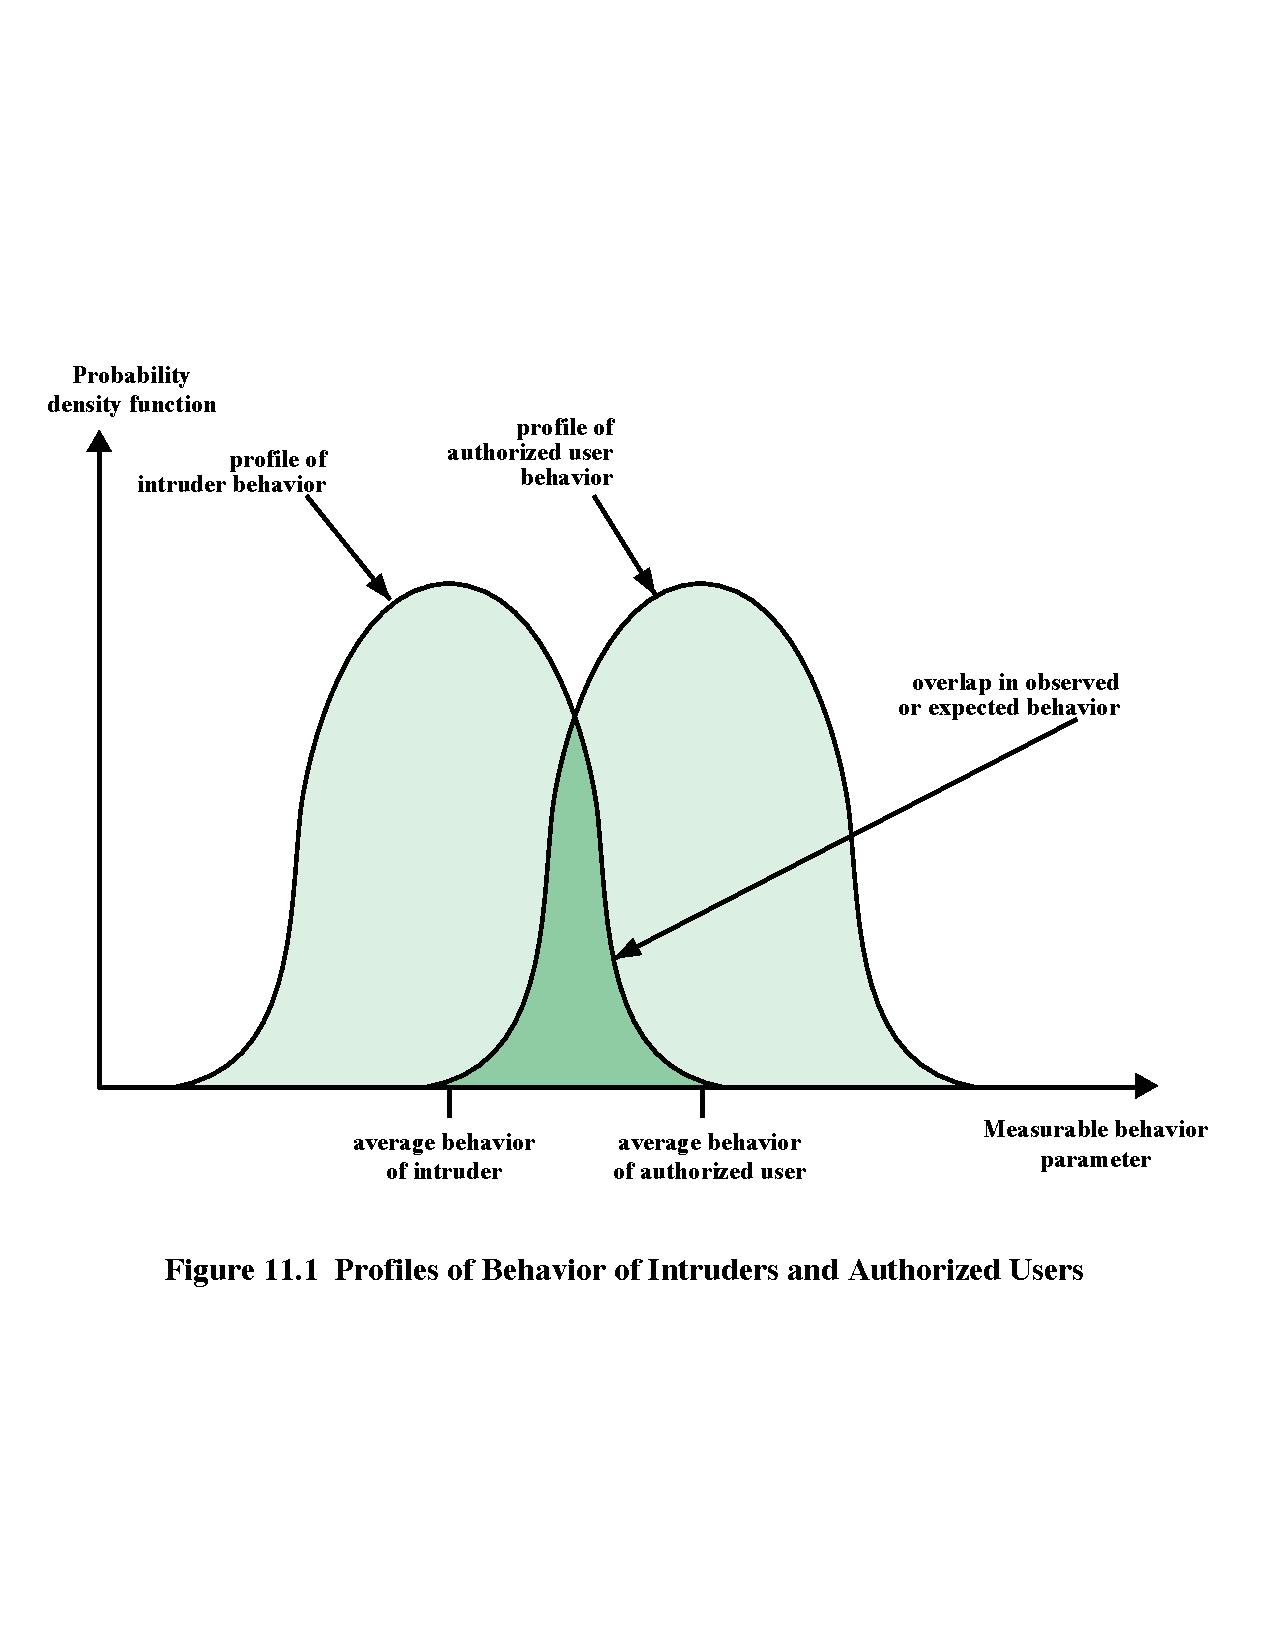
\includegraphics[height=0.7\textheight]{profiles.pdf}
    \caption{User behavioural profiles.
      Image: \cite{Stallings2013nse}.}
  \end{figure}
\end{frame}

\begin{frame}{\insertsubsectionhead}
  \begin{itemize}
    \item False positives: authorised users detected as intruders.
    \item False negatives: intruders detected as legitimate users.

    \item We can reasonably well distinguish masqueraders through past history.

    \item Misfeasors can be detected by defining what's unauthorised use.

    \item Clandestine user is very difficult to detect automatically.

  \end{itemize}
\end{frame}

\subsection{Audit Records}

\begin{frame}{\insertsubsectionhead}
  \begin{itemize}
    \item Native audit records: log all (relevant) user activity using system 
      logs.

    \item Detection-specific audit records: filters out events interesting for 
      the IDS.
      
    \item Example: copying a file.

  \end{itemize}
\end{frame}

\subsection{Statistical Anomaly Detection}

\begin{frame}{\insertsubsectionhead}
  \begin{itemize}
    \item Threshold detection: defining thresholds independent of users.

    \item Profile based: use a profile for each user to detect changes in 
      behaviour.

  \end{itemize}
\end{frame}

\subsection{Rule-Based Intrusion Detection}

\begin{frame}{\insertsubsectionhead}
  \begin{itemize}
    \item Rule-based detection: defines rules for attack patterns, also called 
      signature detection.
  \end{itemize}
\end{frame}

%\subsection{The Base-Rule Fallacy}
%
%\begin{frame}{\insertsubsectionhead}
%\end{frame}

\subsection{Distributed Intrusion Detection}

\begin{frame}{\insertsubsectionhead}
  \begin{figure}
    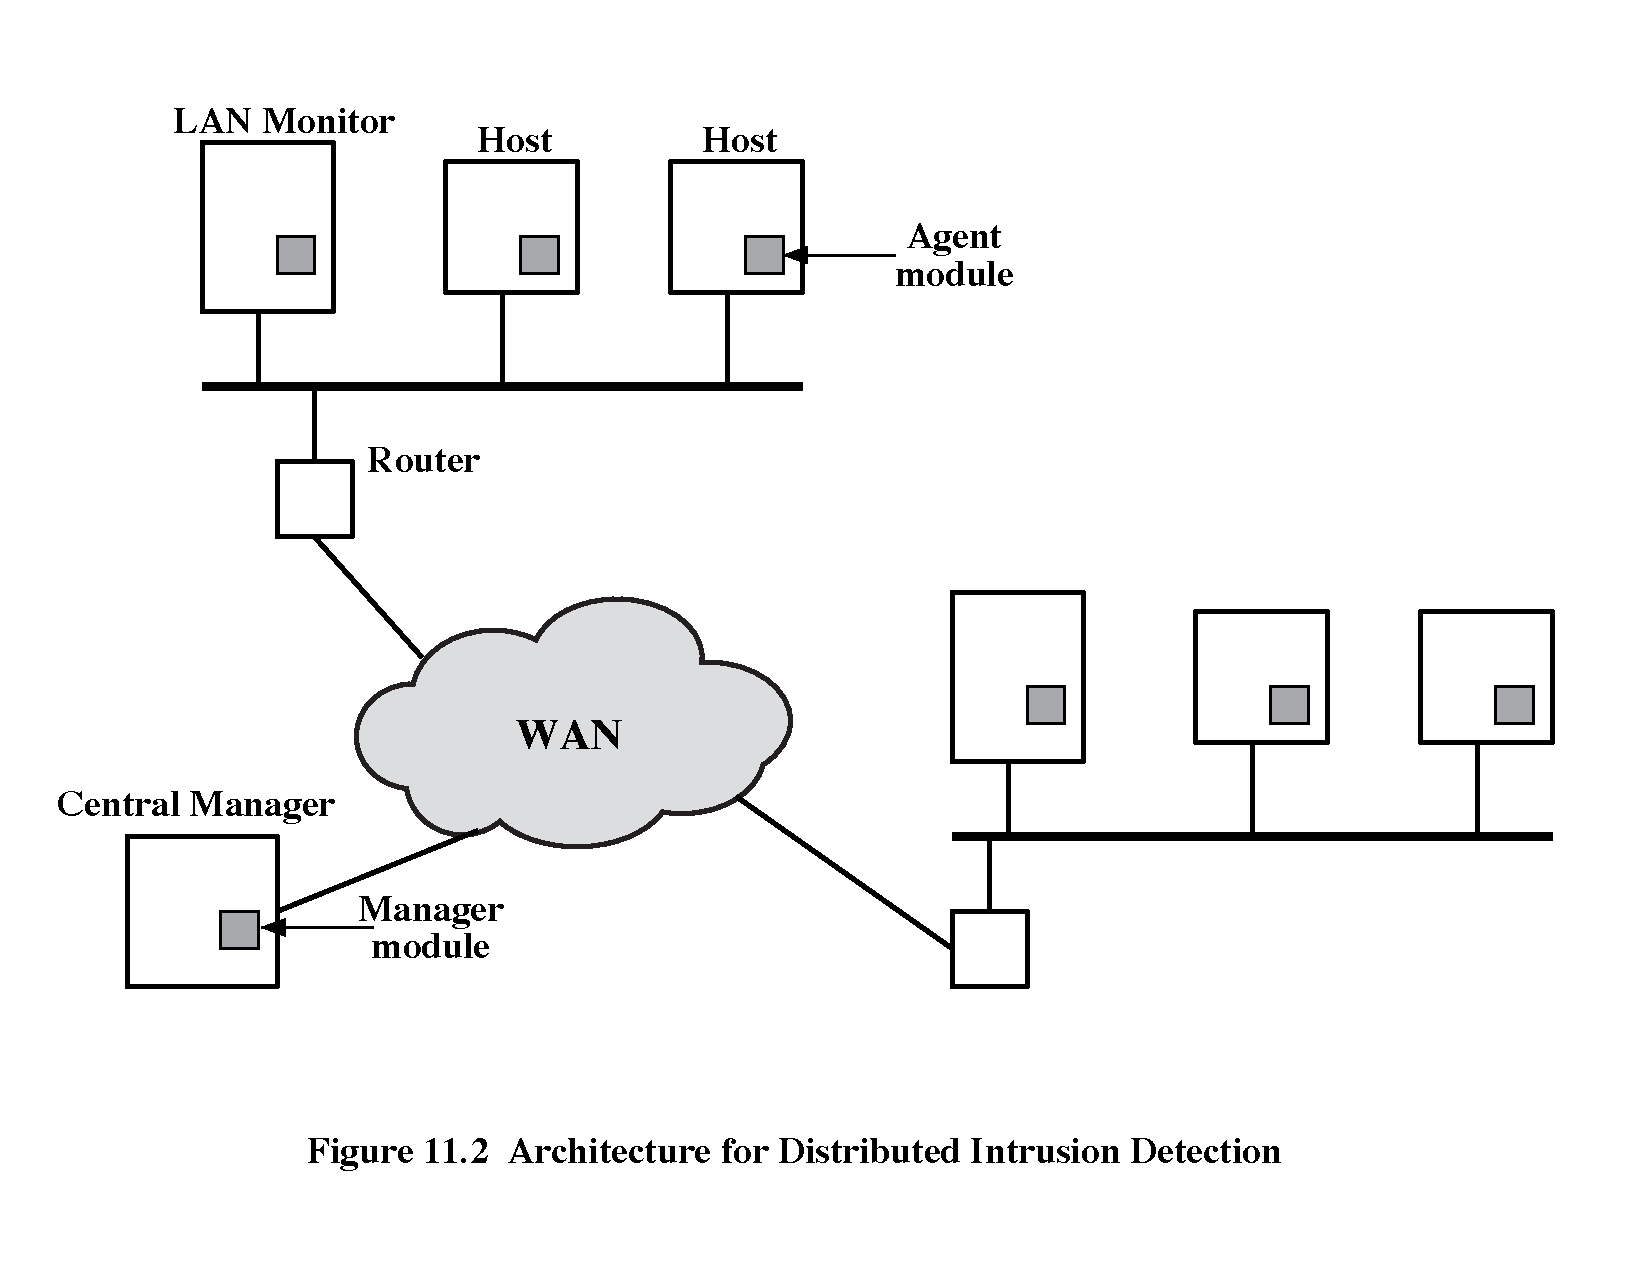
\includegraphics[height=0.7\textheight]{dids.pdf}
    \caption{Distributed Intrusion Detection System.
      Image: \cite{Stallings2013nse}.}
  \end{figure}
\end{frame}

\subsection{Honeypots}

\begin{frame}{\insertsubsectionhead}
  \begin{figure}
    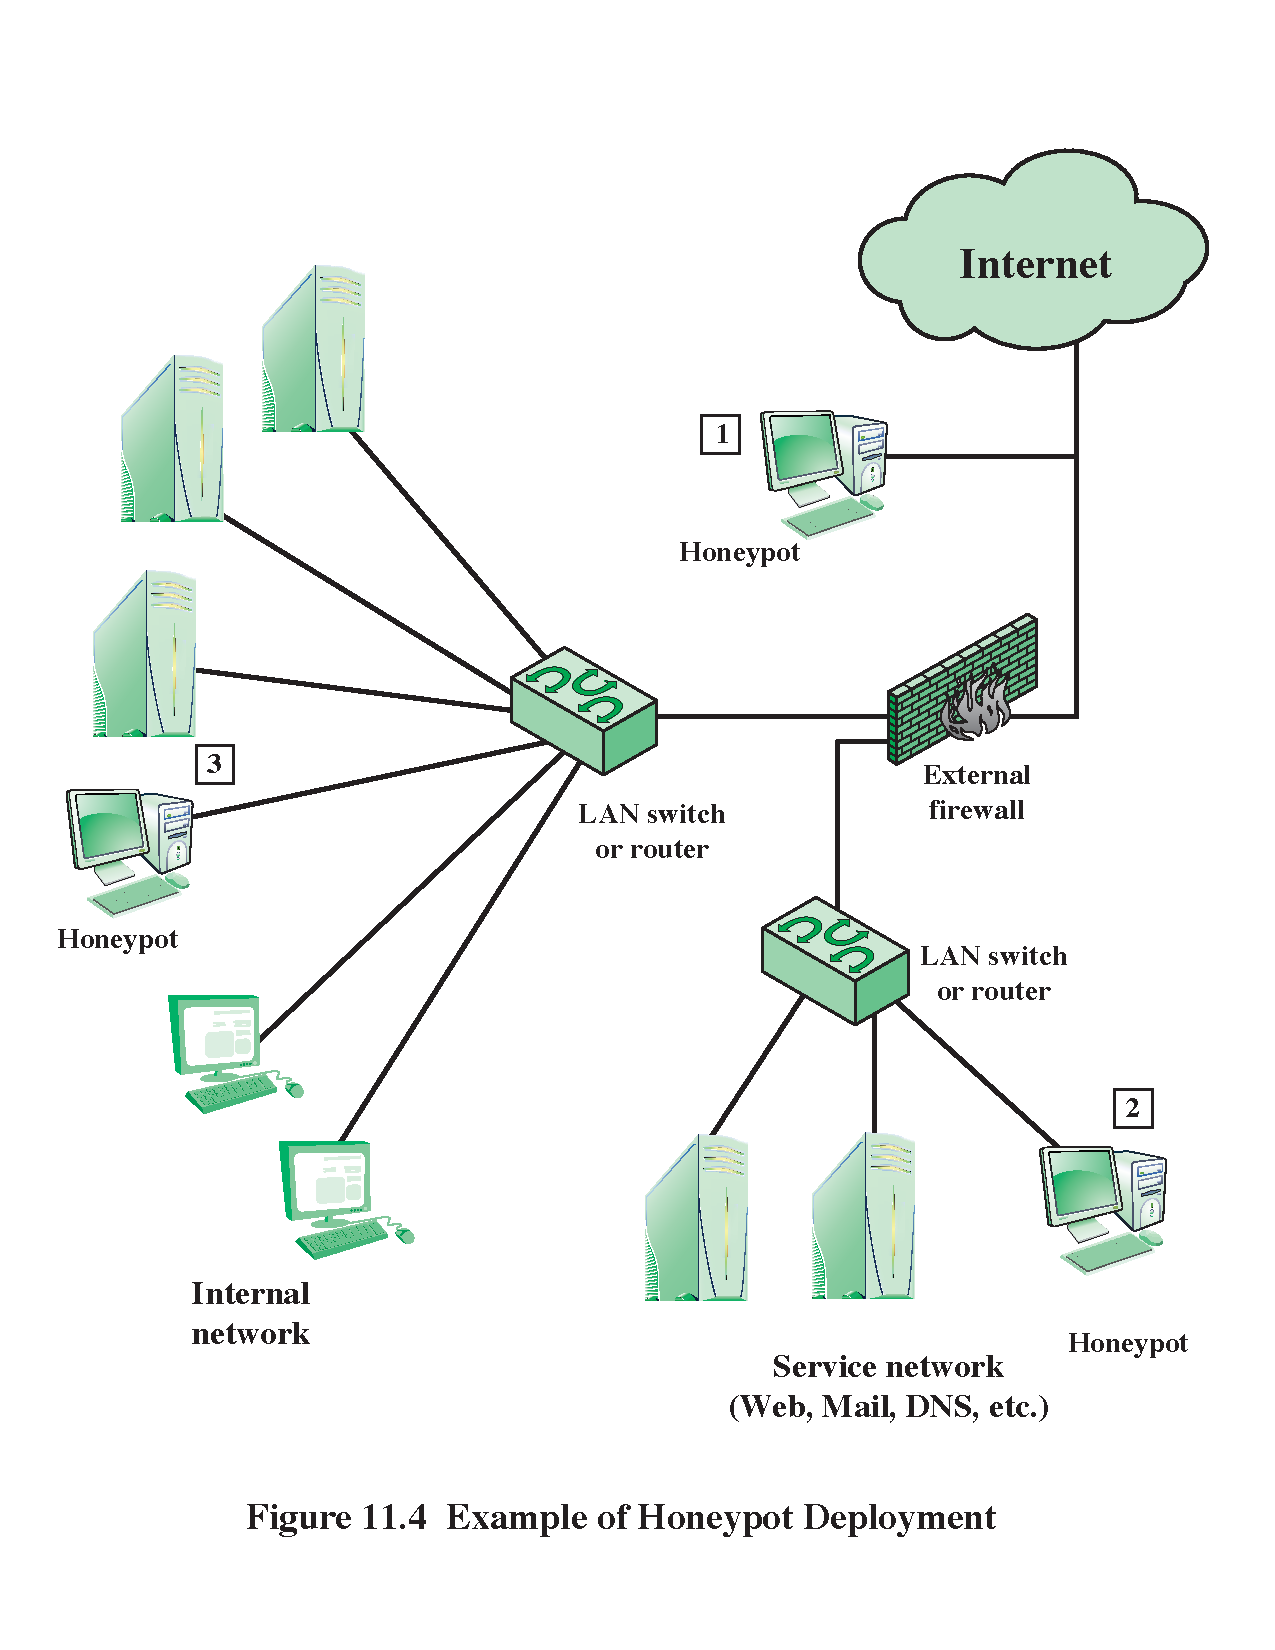
\includegraphics[height=0.7\textheight]{honeypot.pdf}
    \caption{An illustration of honeypots.
      Image: \cite{Stallings2013nse}.}
  \end{figure}
\end{frame}


\section{Password Management}

%\subsection{The Vulnerability of Passwords}
%
%\begin{frame}{\insertsubsectionhead}
%\end{frame}
%
%\subsection{The Use of Hashed Passwords}
%
%\begin{frame}{\insertsubsectionhead}
%\end{frame}
%
%\subsection{User Password Choices}
%
%\begin{frame}{\insertsubsectionhead}
%\end{frame}
%
%\subsection{Password Selection Strategies}
%
%\begin{frame}{\insertsubsectionhead}
%\end{frame}

\subsection{Bloom Filter}

\begin{frame}{\insertsubsectionhead}
\end{frame}



%%%%%%%%%%%%%%%%%%%%%%

\begin{frame}[allowframebreaks]{Referenser}
	\small
  \printbibliography
\end{frame}

\end{document}

